
\section{Introducción}

En esta sección se aborda el proceso de transmisión de información y se analizan las operaciones biológicas que hacen posibles los cómputos en el cerebro. Para empezar a modelar una red neuronal se detallará primero la dinámica de los disparos neuronales.

Recordando los conceptos abordados en el  capítulo  anterior, las neuronas son células especializadas del sistema nervioso central que se comunican mediante señales tanto eléctricas como químicas.  Son células con núcleo, axón y dendritas capaces de transferir impulsos eléctricos. La transmisión de un pulso eléctrico se lleva a cabo desde el soma a través de sus membranas, pasando por los nodos de Ranvier a lo largo del axón, hasta la terminal del axón en los botones sinápticos. Las neuronas hacen sinapsis  permitiendo que el pulso llegue a las dendritas de la neurona postinanáptica, mediante canales iónicos. \parencite{neurona_A_cerebro}

El pulso eléctrico que se desplazo desde el cono axónico de la neurona presináptica hasta la neurona postsináptica, se genera por la diferencia de potencial existente entre el interior y el exterior de la neurona, el cual resulta de las varias concentraciones de iones en ambos lados de la membrana plasmática. Los estados potenciales neuronales presentes en la membrana plasmática del axón se distinguen en los siguientes \parencite{HH}:

\begin{itemize}
\item \textbf{Potencial de reposo:} Se refiere a la diferencia de cargas eléctricas a través de la membrana celular cuando no hay una señal nerviosa en curso. La membrana está polarizada a -70 mV, lo que significa que tiene una carga positiva en el exterior (por la presencia de iones de sodio, Na+) y una carga negativa en el interior debido a iones como el cloruro (Cl-) y proteínas. En este estado, la membrana no transmite señales nerviosas. Ver la figura \fref{fig:MembranaP} lado derecho.

\item \textbf{Potencial de acción o membrana:}  Se produce cuando un estímulo alcanza un nivel umbral de 55 mV. Este evento despolariza la membrana, lo que significa que cambia rápidamente su polaridad de negativa a positiva. Esto ocurre porque se abren canales de iones de sodio (Na+) y potasio (K+), permitiendo el flujo de estos iones a través de la membrana, ver la figura \fref{fig:MembranaP} lado izquierdo. Este cambio rápido en la polaridad de la membrana es lo que impulsa el avance de la señal nerviosa. Las etapas del potencial de acción está representado en la figura \fref{fig:graficaP}
\end{itemize}


\begin{figure}[h]
 \centering
 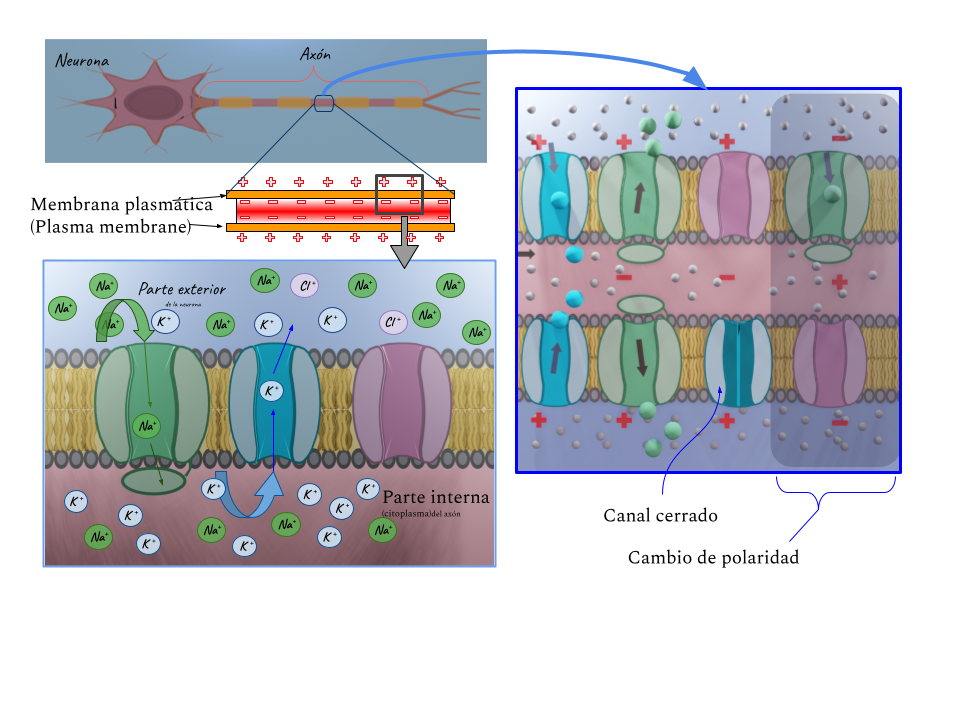
\includegraphics[scale=0.5]{../Figuras/MembranaP.png}
 \caption{Representación de la membrana axónica en potencial de reposo en la parte inferior izquierda, y en la parte derecha con un estímulo que genera el cambio de polaridad en la misma, así como el cierre de canales y paso de iones.}
 \label{fig:MembranaP}
\end{figure}

\begin{figure}[h]
 \centering
 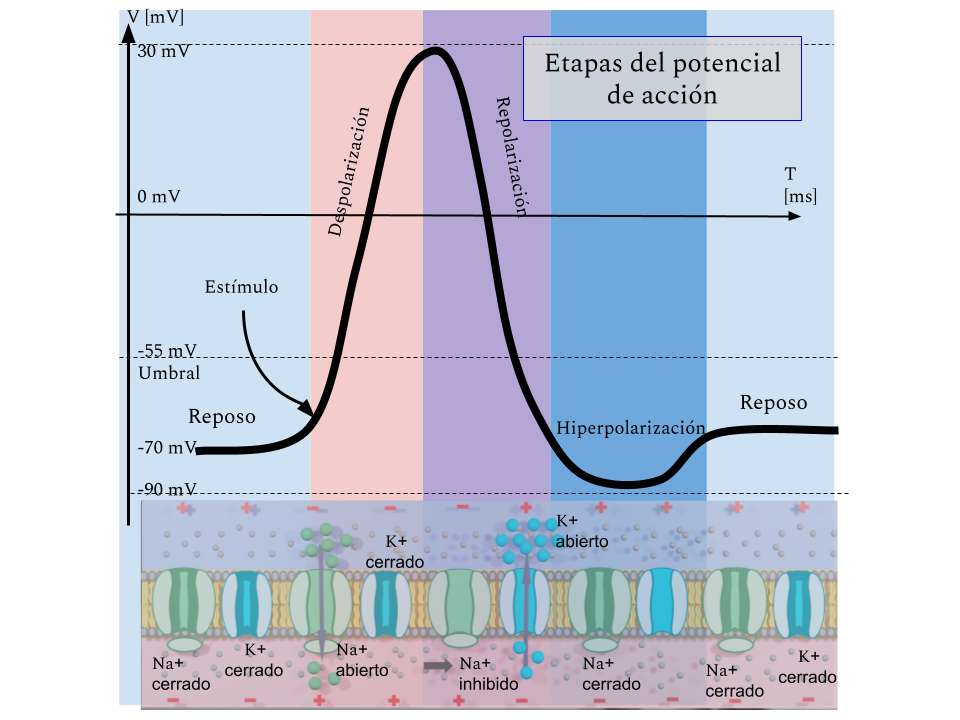
\includegraphics[scale=0.5]{../Figuras/Grafica.png}
 \caption{Representación gráfica de la respuesta de los canales iónicos de sodio (Na+ en verde) y potasio (K+ en azul) ante un estímulo de voltaje, dando como resultado un potencial de acción que viajará a lo largo de todo el axón.}
 \label{fig:graficaP}
\end{figure}

Los pioneros en el estudio del potencial de acción y elaboración de un modelo para la unión sináptica eléctrica fueron Alan Lloyd Hodgkin y Andrew Fielding Huxley alrededor de 1952. Este modelo matemático, intentaba esclarecer los procesos neuronales, surgió a partir de investigaciones experimentales  \footnote{El texto original de este experimento se puede encontrar en la siguiente url: \url{ https://physoc.onlinelibrary.wiley.com/doi/pdf/10.1113/jphysiol.1952.sp004764}}.

Estos científicos llevaron a cabo sus estudios utilizando un calamar gigante, un animal que puede alcanzar hasta 4 metros de longitud y posee un axón a proporción, que se extiende casi a lo largo de la mitad del cuerpo del calamar y tiene un grosor de medio milímetro, en comparación con el tamaño estándar del axón de una neurona, que oscila entre 1 y 20 micrómetros. 
El axón del calamar gigante es tan grande que les permitió introducir dispositivos para medir el voltaje, es decir, la diferencia de potencial entre el interior y exterior de la neurona. Con estas mediciones experimentales, lograron determinar las dinámicas de las cargas eléctricas tanto en el interior como en el exterior de la neurona, lo que facilitó el estudio de la transferencia de electricidad durante la activación de un impulso nervioso.
 

\section{Membrana y canal}

Durante las observaciones del flujo de corrientes eléctricas el sistema parecía comportarse como un circuito eléctrico, donde la membrana actuaba como un componente poroso que \textit{funciona como un capacitor}, almacenando ligeramente las cargas cuando intentan pasar de un lado a otro. Además esta membrana tiene la cualidad de permitir el paso selectivo de iones en ciertos momentos, es decir es una estructura \textit{semipermeable} que se representa con \textit{resistencias variables}. Ver Figura \ref{fig:ModelHh}.

Los canales de iones permiten o bloquean el flujo de iones dependiendo de la diferencia de potencial que exista entre el interior y el exterior de la membrana y de su estado de reposo particular. Por tanto es necesario agregar los potenciales de reposo para cada canal al modelo, en la figura \ref{fig:circuito} se agregan.


\begin{figure}[h]
 \centering
 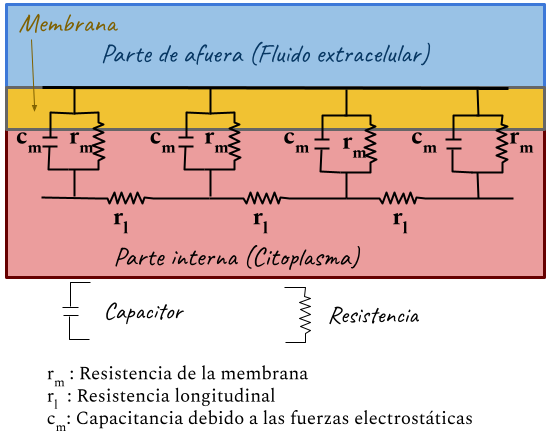
\includegraphics[scale=0.5]{../Figuras/ModeloHH.2}
 \caption{Un primer modelo de la membrana axónica modelada como circuito eléctrico.}
 \label{fig:ModelHh}
\end{figure}



\begin{figure}[h]
 \centering
 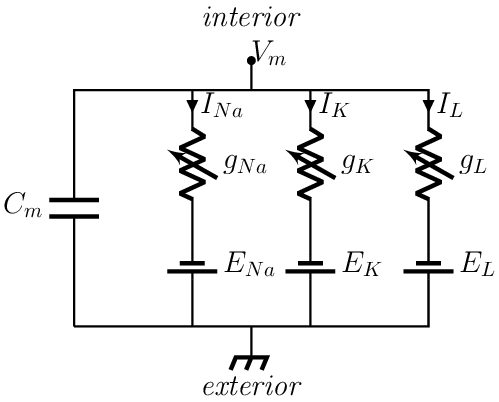
\includegraphics[scale=0.5]{../Figuras/circuito.png}
 \caption{Modelo de la membrana axónica modelada como circuito eléctrico, con los distintos canales presentes y sus voltajes en reposo.}
 \label{fig:circuito}
\end{figure}

Los elementos necesarios para el modelo de la membrana son los siguientes:
\begin{itemize}
\item Potenciales eléctricos \emph{E ó  V}; Se mide en \emph{mV}.
    \begin{itemize}
     \item \emph{E\textsubscript{(Na,K,L)}} 
     Potencial de equilibrio o reposo para los iones de sodio (Na), potasio (K) y cloruro y de fuga (L). 
     \begin{itemize}
        \item E \textsubscript{Na}  \emph{50mV}
        \item E \textsubscript{Ca}  \emph{150mV}
        \item E \textsubscript{K}   \emph{- 80mV}
        \item E \textsubscript{Cl}  \emph{- 60mV}
        \end{itemize}

     \item \emph{V\textsubscript{m}} Potencial eléctrico de la membrana. 
     \end{itemize}

\item Corriente \emph{I}; Movimiento de cargas. Se mide en \emph{µA}.
    \begin{itemize}
     \item \emph{I\textsubscript{(Na,K,L)}} corriente entrante a los canales de Na, K o L.
     \end{itemize}

\item Resistencia \emph{R}; Medida de la oposición al movimiento de las partículas cargadas.
\item Capacitancia o capacidad eléctrica \emph{C} . Cantidad de energía eléctrica almacenada en un capacitor para una diferencia de potencial eléctrico dada.
    \begin{itemize}
     \item \emph{C\textsubscript{m}} la capacitancia de la membrana. 
     \end{itemize}

\item Conductancia \emph{g}; Inverso de la resistencia \( \dfrac{1}{R} \) , es decir, facilidad de transmisión de las partículas cargadas.
    \begin{itemize}
     \item \emph{g\textsubscript{(Na,K,L)}}  la conductancia del canal de sodio, potasio, cloro y fuga. 
     \end{itemize}

\end{itemize}

\section{Modelo de los canales de inoes}

En la figura \fref{fig:MembranaP} se puede ver la representación de membrana y sus lipidos, la carga es almacenada en la membrana por un breve periodo de tiempo, dando como resultado que la bicapa se comporte como un \textbf{capacitor}. Esta membrana también está con cierta resistencia al paso de corriente representado en el diagrama \ref{fig:circuito} \footnote{Otra explicación más detallada la podemos encontrar en \url{https://neurowiki.case.edu/wiki/Action_Potential_IV:_Hodgkin-Huxley_Equations_and_Other_Conductances}} 

La membrana de una neurona es modelada como un elemento de un circuito con capacitancia \emph{C\textsubscript{m}} y potencial \emph{V}, las corrientes que fluye a través de la bicapa lipídica están regidos por las siguientes ecuaciones:

\begin{equation}
  I_{m} = C_{m} \dfrac{dV_{m}}{dt}
  \label{eq:corrientesEnLaMembrana}
\end{equation}


\begin{equation}
  C_{m} \dfrac{dV_{m}}{dt} =  - g_{Na} m^3 h(V - E_{Na} ) - g_{K} n^4 (V - E_{K} ) - g_{L} (V - E_{L} ) + I_ext
  \label{eq:corrientesEnLaMembrana2}
\end{equation}

\begin{equation}
  \dfrac{1}{\gamma(T)}\dfrac{dn}{dt} =  \alpha_{n^\infty} (V)(1 - n) - \beta_{n} (V) n = \dfrac{n(V)-n(t)}{\tau_{n}(V)}
  \label{eq:corrientesEnLaMembrana3}
\end{equation}

\begin{equation}
  \dfrac{1}{\gamma(T)}\dfrac{dm}{dt} =  \alpha_{m} (V)(1 - m) - \beta_{m} (V) m = \dfrac{m^\infty(V)-m(t)}{\tau_{m}(V)}
  \label{eq:corrientesEnLaMembrana4}
\end{equation}

\begin{equation}
  \dfrac{1}{\gamma(T)}\dfrac{dh}{dt} =  \alpha_{h} (V)(1 - h) - \beta_{h} (V) h = \dfrac{h^\infty(V)-h(t)}{\tau_{h}(V)}
  \label{eq:corrientesEnLaMembrana5}
\end{equation}

La ecuación principal es \ref{eq:corrientesEnLaMembrana} que donde la corriente de la membrana está dada por su capacitancia con el cambio voltaje en la membrana respecto al tiempo.


\begin{definition}
 \emph{Canal persistente} Tiene un solo tipo de compuerta y dos estados posibles:
 \begin{enumerate}
  \item \textbf{Activado}
  \item \textbf{Desactivado}
 \end{enumerate}

\end{definition}

\begin{definition}
 \emph{Canal transitorio} Tiene compuertas de activación e inactivación, y tres estados:
 \begin{enumerate}
  \item \textbf{Activado} Ambas compuertas abiertas.
  \item \textbf{Desactivado} Compuerta de activación cerrada, inactivación abierta.
  \item \textbf{Inactivado} Compuerta de inactivación cerrada.
 \end{enumerate}

\end{definition}




Cada una de las partes del lado izquierdo de la ecuación \ref{eq:corrientesEnLaMembrana2} corresponde a las compuertas de los canales y la corriente de un estímulo escrictamente externo que pueda influir a la membrana.

De manera sencilla podemos notar al canal de potasio como una puerta hecha de cuatro subpuertas por donde los elementos pasan o no pasan, es decir tiene dos estados; activado o desactivado. El canal de sodio lo podemos notar como una puerta que está hecha de tres subpuertas del mismo tipo por donde los elementos pasan o no pasan y tiene aparte un tapón extra, que hace que aunque estas tres están abiertas bloquee toda la compuerta, es decir tiene tres estados; desactivado, activado, inactivo. Con esto podemos representar a las conductancias \textbf{G} como:

\begin{itemize}
 \item \({G_{Na}} = g_{Na} * m ^3 * h \) donde \(g_{Na}\) es una constante que representa el valor de la conductancia máxima/\(cm ^2\), \textbf{m} es la proporción de los canales de sodio abiertos (representa la concentración de sodio) y nos indica la activación (subpuertas abiertas) del canal, \textbf{h} es el “tapón” de la compuerta que puede impedir el paso de iones independientemente de las otras tres subpuertas, es decir la inactivación (compuerta bloqueada).
Los movimientos combinados de \textbf{m} y \textbf{h} son los que controlan la compuerta de sodio.
 \item \({G_{K}} = g_{K} * n^4\) donde \(g_{K}\) es una constante que representa el valor de la conductancia máxima /\(cm^2\), \textbf{n} es la proporción de los canales de potasio abiertos (representa la concentración de potasio) y nos indica la activación del canal de potasio.
 \item \(g_{L}\) es una constante, de los canales por fuga, que representa la concentración de los demás iones que pasan por la membrana.
\end{itemize}

Las concentraciones de iones están dado por \emph{m}, \emph{n} y \emph{h}, que son variables de activación que describen la probabilidad de que los canales iónicos estén abiertos. Donde la ecuación \ref{eq:corrientesEnLaMembrana3} representa las subpuertas del canal de potasio y las ecuaciones \ref{eq:corrientesEnLaMembrana4} y \ref{eq:corrientesEnLaMembrana5} representando cada una un tipo de subpuerta al canal de sodio.

Cada elemento en las ecuaciones \ref{eq:corrientesEnLaMembrana3}, \ref{eq:corrientesEnLaMembrana4}, \ref{eq:corrientesEnLaMembrana5} con \(ion\) denotando las compuertas del potasio \(n\) o del sodio, ya sea \(m\) o \(h\) se describen se la siguiente forma \parencite{HH52}:

\begin{itemize}
 \item \(\dfrac{1}{\gamma(T)}\) Es el coeficiente de escala temporal, dependiente de la temperatura. Para efectos prácticos se considera constante.
 \item \(\alpha_{ion}(V)\) Es la probabilidad de que una compuerta transite de cerrada a abierta.
 \item \(\beta_{ion}(V)\) Es la probabilidad de que una compuerta transite de abierta a cerrada.
 \item \(ion^\infty(V)\) Es la probabilidad que la compuerta del ion n, m ó h quede abierta en el estado de equilibrio cuando \(t \rightarrow \infty\).
 
 \item \(\tau_{ion}(V)\) Tiempo que toma llegar al equilibrio.
\end{itemize}

Las expresiones de \(\alpha\) y \(\beta\) están dadas por las siguientes ecuaciones:

\begin{align*}
\alpha_{n}&=\dfrac{0.01(10-V)}{exp(\dfrac{10-V}{10})-1}           &  \beta_{n}&=0.125exp-\dfrac{V}{80}\\
\alpha_{m}&=\dfrac{0.01(25-V)}{exp(\dfrac{25-V}{10})-1}                    &  \beta_{m}&=4exp-\dfrac{V}{18}\\
\alpha_{h}&=\dfrac{0.07}{exp-(\dfrac{V}{20})}              &  \beta_{h}&=\dfrac{1}{1+exp\dfrac{30-V}{10}}
\end{align*}

Los factores \(\alpha\) y \(\beta\) se denominan como constantes de velocidad de transición. Donde \(\alpha\) es el número de veces por segundo que se abre una puerta que está en estado cerrado, mientras que \(\beta\) es el número de veces por segundo que se cierra una puerta que está en estado abierto. Si la membrana tiene un la carga negativa, \(\alpha\) debe aumentar y \(\beta\) debe disminuir, cuando la membrana esté despolarizada.

\subsection{Estados de la membrana}

Los estados de la membrana están dados por estados electroquímicos que determinan su potencial eléctrico y paso de iones, son los siguientes: 

\begin{enumerate}
 \item \textbf{Estado Polarizado:} En su estado de reposo tiene \(V < 0 ( V \approx -70 mV )\).
 \item \textbf{Estado Despolarizado:} Es cuando \(V \geq 0\).
 \begin{itemize}
  \item Se pasa a este estado cuando en las dendritas y en el cuerpo de la neurona se acumula una carga muy grande (un voltaje eléctrico, disparo), lo que desencadena la apertura del canal de sodio. 
  \item Iones positivos de sodio entran a la membrana. 
 \end{itemize}
 \item \textbf{Estado Hiperpolarizado:} Es cuando \(V << 0\).

  \begin{itemize}
    \item Tras la despolarización los distinto tipos de canales iónicos buscan restaurar a la neurona a su estado de reposo.
    \item Los canales de potasio abren sus compuertas, provocando que salga el potasio que está dentro del axón. 
    \item Iones de potasio positivos salen de la membrana.
    \item Se incrementa la polaridad negativa de la membrana disminuyendo aún más el potencial eléctrico.
    \item Un breve lapso la neurona se inactiva eléctricamente, evitando que se genere un nuevo impulso eléctrico hasta que regrese a su estado de equilibrio, fenomeno conocido como
    periodo de refracción.
 \end{itemize}

\end{enumerate}
 
\section{Simulación del disparo de una neurona usando el método de Euler}

Los estados de la membrana se obtuvieron haciendo la simulación de un disparo neuronal, también conocido como spike. Se modelaron utilizando el Método de Euler para resolver las ecuaciones diferenciales que describen el fenómenos neuronal \footnote{Hodgkin-Huxley Simulation Using Euler's Method lo puedes encontrar en la siguiente liga \url{https://webpages.uidaho.edu/rwells/techdocs/Biological\%20Signal\%20Processing/Chapter\%2003\%20The\%20Hodgkin-Huxley\%20Model.pdf}}. A continuación, se describe con detalle el proceso y los pasos involucrados en la aplicación del Método de Euler para la simulación de disparos neuronales:

\begin{algorithm}
  \caption{Algoritmo de integración de Euler [Wells pp51].}\label{AIE}
  \begin{algorithmic}[1]
    \Function{INTEGRADISPARO}{$T,\Delta T,V_{0},I_{ext}(t)$}
    \State Inicializar arreglos de longitud T: $T[],V[],n[],m[],h[],G_{Na}[],G_{K}[],\tau_{n}[],\tau_{m}[],\tau_{h}[] \gets arreglo[numeroDePasos] $
    \State  $V[0] \gets V_{0}$
    \For {$ t = 0  a  t = T cada \Delta t $}
        \State Calcular $\alpha_{n}, \beta_{n}, \alpha_{m}, \beta_{m},\alpha_{h}, \beta_{h} $ utilizando $V(t)$.
        \State Calcular las tres $\tau_{x} $ y $x^\infty $ apartir de las anteriores.
        \State Calcular las probabilidades de las compuertas $n, m, h, $ utilizando las ecuaciones en diferencias en su forma matricial $\Pi(t + \Delta t) = A_{\pi}\Pi(t) + B_{\pi}$.
        \State Calcular $G_{Na} = g_{Na}m^3h $ y $G_{K} = g_{K}n^4 $.
        \State Almacenar los resultados de este paso en los arreglos $T[], V[], n[], m[], h[], G_{Na}[], G_{K}[], \tau_{n}[], \tau_{m}[], \tau_{h}[] $
        \State $I_{ext} \gets I_{ext}(t) $
        \State Calcular $V_{m} (t + \Delta t) $
    \EndFor
    \State Devolver los arreglos $T[],V[],n[],m[],h[],G_{Na}[],G_{K}[],\tau_{n}[],\tau_{m}[],\tau_{h}[] $ con los resultados para los tiempos $[0,T] $
    \EndFunction
  \end{algorithmic}
\end{algorithm}

Los valores que necesita el algoritmo de intergración de Euler son los siguientes:

\begin{enumerate}
 \item $T$:  Asigna durante cuánto tiempo correrá la simulación.
 \item $\Delta T $: Asigna que tan cortos serán los intervalos. Se necesita aproximar la función con segmentos de recta siguiendo la tangente. 
 \item $V_{0} $: El voltaje inicial.
 \item $I_{ext}(t) $: La corriente externa.
\end{enumerate}

Una vez inicializados los valores para las conductancias, las probabilidades de la apertura de los canales y los estados de equilibrio para cada canal. Se pasa a calcular las probabilidades del cambio de estado de las compuertas de los canales, es decir 
 las alfas y betas. Es entonces que se puede calcular el tiempo que retoma el equilibrio, es decir las $\tau$ , $n^{\infty}$, $m^{\infty}$, $h^{\infty}$. Se calculan las probabilidades de las compuertas n, m, h usando las ecuaciones diferenciales en forma matricial, de la forma dada en la figura \fref{fig:matriX}. En estos calculos se puede presentar el problema de truncamiento y llegar a resultados muy distantes de los esperados.


\begin{figure}[H]
 \centering
 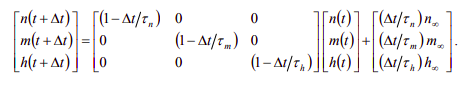
\includegraphics[scale=0.7]{../Figuras/matrix.png}
 \caption{Forma matricial para el cálculo de las probabilidades de las compuertas n, m, h.}
 \label{fig:matriX}
\end{figure}

Una vez computado las probabilidades, se asigna las conductancias sustituyendo los valores respectivos. Por razones de analisis en caso de obtener valores inesperados se almacenan los \emph{resultados temporales}. Se actualiza la corriente externa deacuerdo a los valores siguientes en el tiempo a calcular.

El algoritmo es iterativo así que se reperitan los pasos descritos para cada tiempo t, conforme avance el tiempo, obtenemos los valores del voltaje. Terminando el tiempo asignado a la simulación, tenemos ya los arreglos llenos de los datos que nos van a poder permitir graficar, que sucedió en cada tiempo para cada canal. 

Las gráficas que se obtuvieron experimentalmente se encuentran en el texto A QUANTITATIVE DESCRIPTION OF MEMBRANE CURRENT AND ITS APPLICATION TO CONDUCTION AND EXCITATION IN NERVE BY A. L. HODGKIN AND A. F. HUXLEY \parencite{HH52}

